
%(BEGIN_QUESTION)
% Copyright 2009, Tony R. Kuphaldt, released under the Creative Commons Attribution License (v 1.0)
% This means you may do almost anything with this work of mine, so long as you give me proper credit

Use loop simulation software on a personal computer to simulate the effects of an ``open loop'' test.  This means placing the loop controller in manual mode and moving the control valve by 5\% or 10\%.  Try this on a simulated process of your own choosing (browse the software's available process types) and sketch the results:

$$\includegraphics[width=15.5cm]{i04326x01.eps}$$

Determine whether the process possesses one or more orders of {\it lag}, and estimate both the time constant of the process and the dead time of the process.

\vskip 10pt

Multiple lags? \underbar{{\it Yes} or {\it No}} \hskip 30pt Time constant = \underbar{\hskip 50pt} \hskip 30pt Dead time = \underbar{\hskip 50pt} 


\vskip 20pt \vbox{\hrule \hbox{\strut \vrule{} {\bf Suggestions for Socratic discussion} \vrule} \hrule}

\begin{itemize}
\item{} What characteristics of the open-loop trend would you inspect to determine whether or not a process has {\it multiple} lags?
\item{} Explain the significance of multiple lags in a process.  How does this impact our ability to control the process using negative feedback (a loop controller)?
\item{} Explain the significance of dead time in a process.  How does this impact our ability to control the process using negative feedback (a loop controller)?
\item{} Generally speaking, which is worse for feedback control: a relatively large {\it lag} time or a relatively large {\it dead} time?  Explain your reasoning.
\end{itemize}

\underbar{file i04326}
%(END_QUESTION)





%(BEGIN_ANSWER)


%(END_ANSWER)





%(BEGIN_NOTES)

%INDEX% Control, process characteristics: computer simulation software (lag and dead times)

%(END_NOTES)

